\section{Ongoing Developments}

The software framework and event reconstruction described in the previous sections are based on the code that
is currently being utilized for data processing or will be deployed in the near future in a upcoming release.
Nevertheless, as CLAS12 data are being analyzed, several potential improvements have been identified and are
either in the process of being implemented or planned for the near future. In this section, we discussed the most
relevant developments.

\subsection{Artificial Intelligence Assisted Forward Tracking}

Recent progress in the field of machine learning offers a promising alternative to conventional algorithmic tracking
methods. While the conventional methods provide algorithms that are well understood and well studied, there are
some algorithms in the data reconstruction process that can be substituted with neural networks to reduce data
processing times. For CLAS12, tracking is the most time-consuming aspect of experimental data processing.
Tracking in the DC takes up to $\sim$90\% of the total data processing time, which includes finding track
candidates and iterating through track-forming segments to find the best combinations of segments that can form
a track. This time increases with luminosity as the number of noise segments increases and can ultimately lead to
processing time degradation. We have started to address this issue by employing machine learning techniques
to find the best track candidates in each event and to reduce the number of combinatorics.

With increased luminosity, the number of potential DC cross candidates increases. This implies that the Kalman
Filter fitting algorithm must be run for all possible combinations of crosses. Figure~\ref{fig:nn1} shows a typical
example of DC data in a projective view using {\it ced}. This figure illustrates the potential of combinatorial trials
to identify tracks. We are developing a classifier convolutional neural network that can identify which segments
from each region of the DCs can potentially form a good track. We intend to use this network in reconstruction
processing to reduce the number of combinatorial fits.

\begin{figure}
\centering
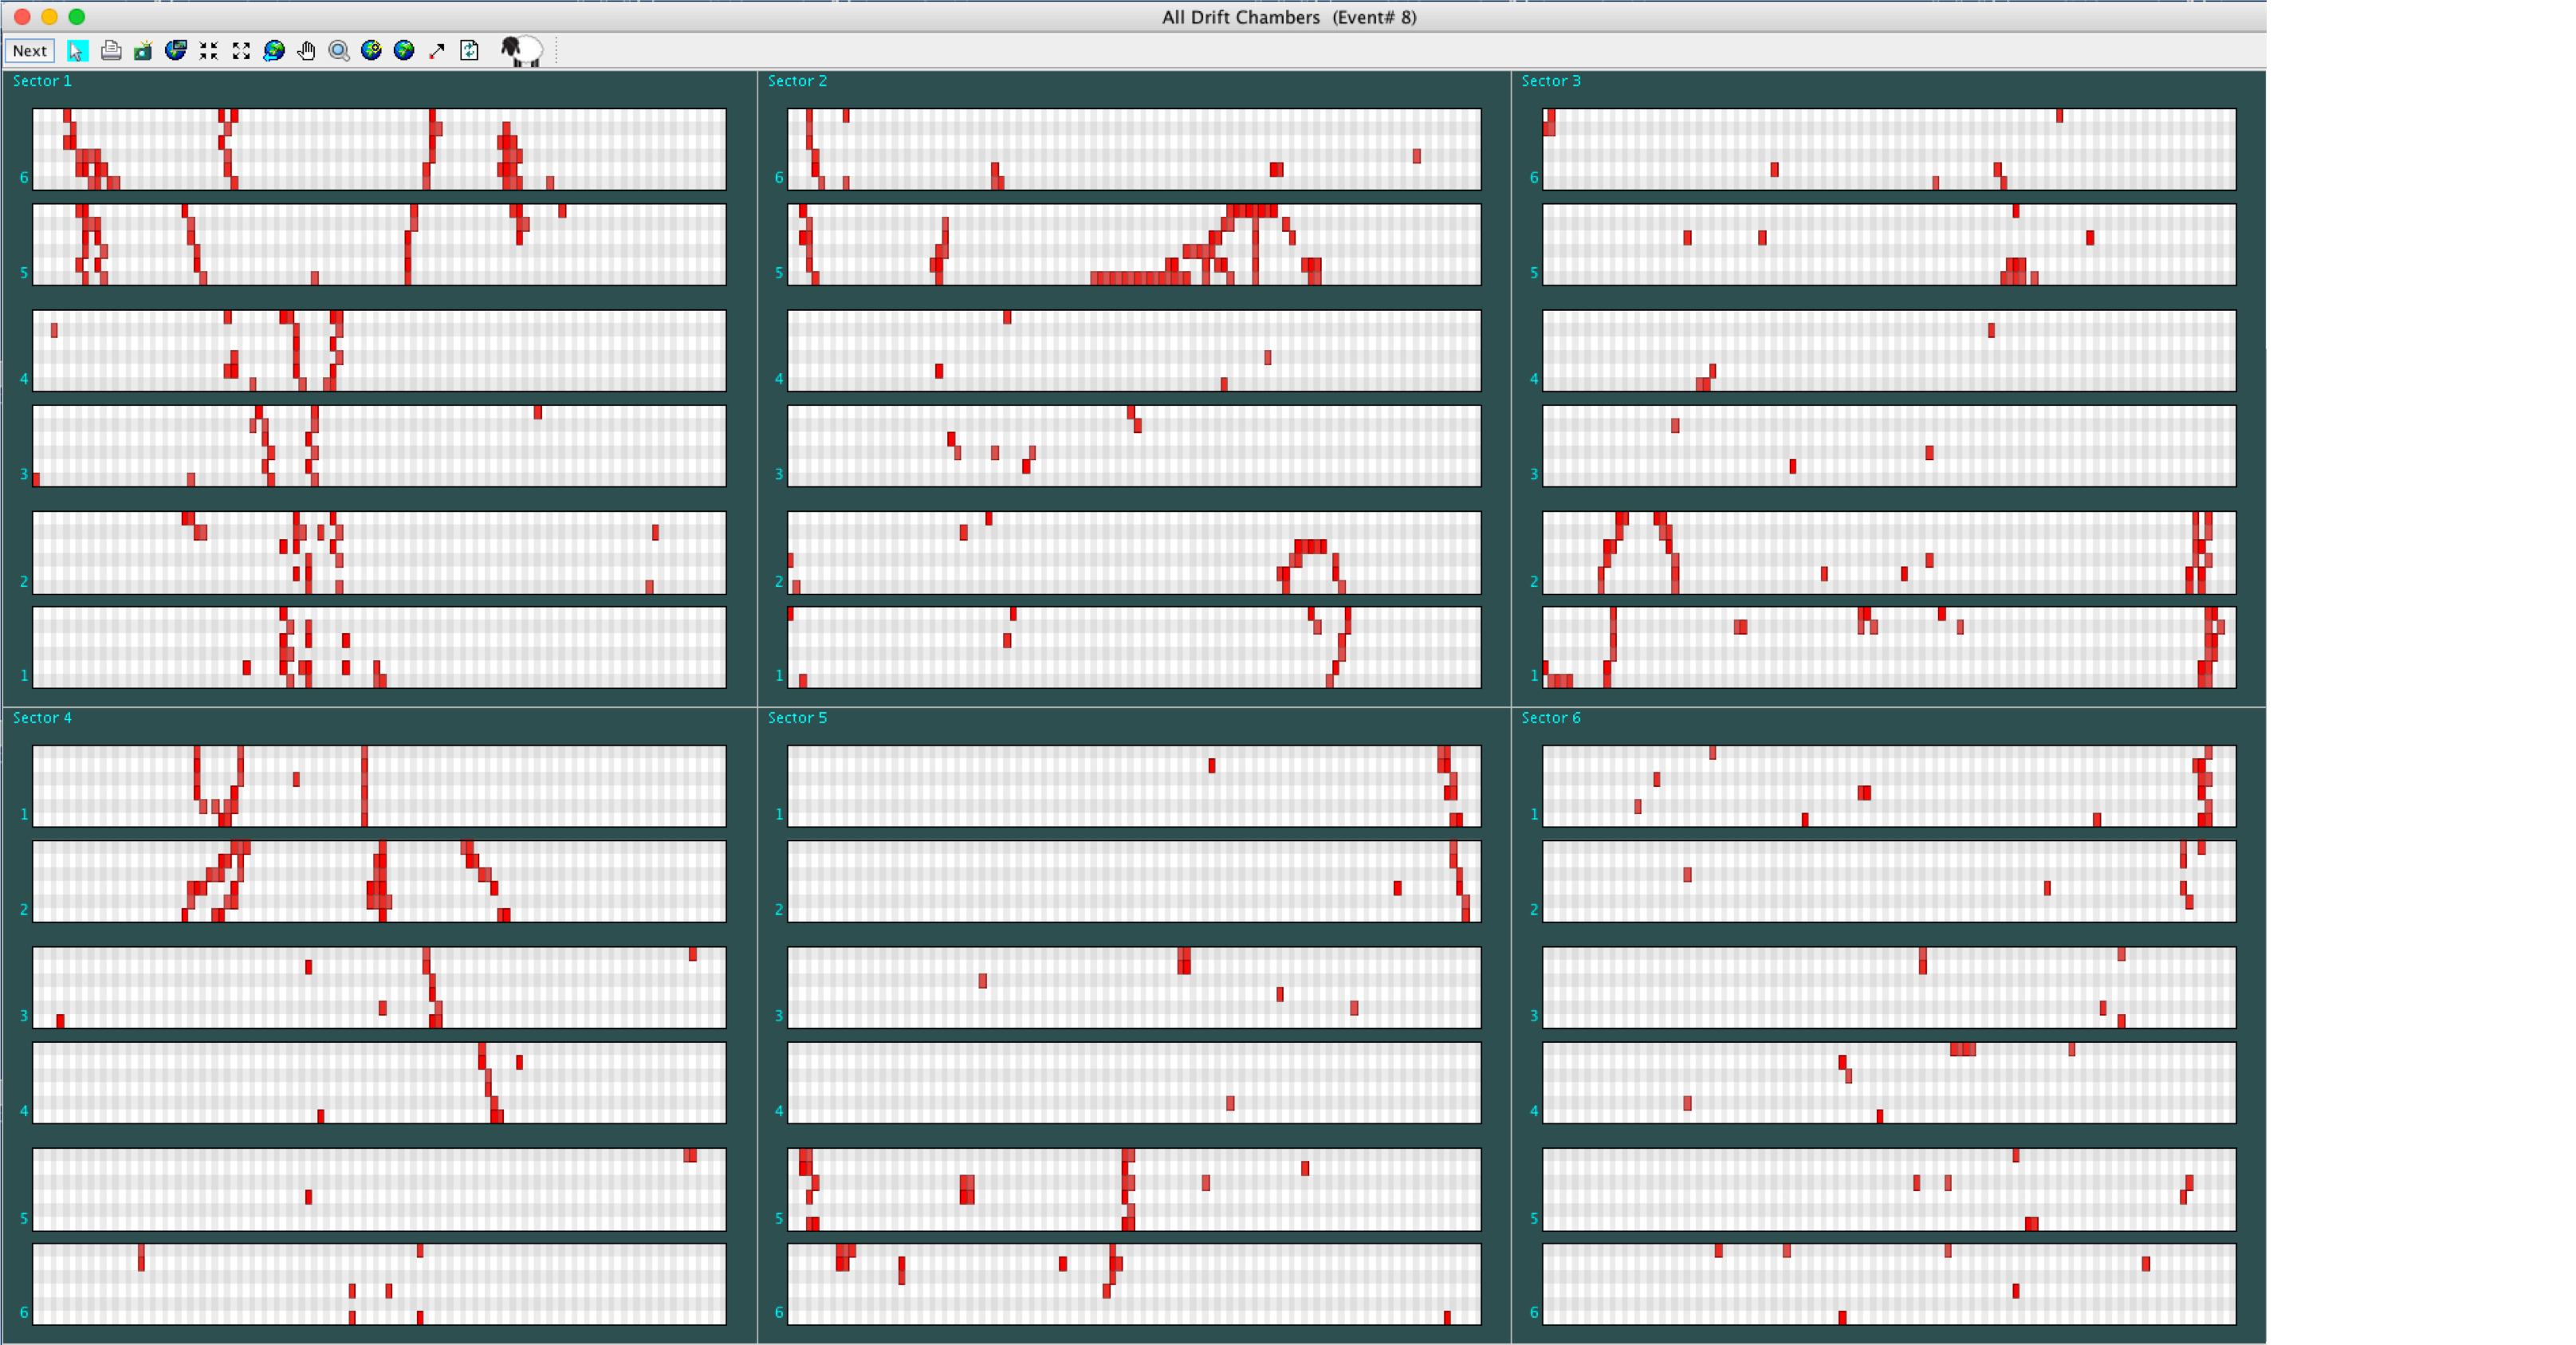
\includegraphics[width=0.53\textwidth]{pics/nn1.png}
\caption{Event display from {\it ced} of track segments in the DC for a typical beam event during data taking
  at the nominal CLAS12 luminosity. This display shows the six DC superlayers in each sector of the Forward
  Detector. Each superlayer contains six layers of 112 wires. Each wire cell is represented by an square cell on the
  display. A wire with a hit is colored in red.}
\label{fig:nn1}
\end{figure}

Reconstructed track segments from both positive and negative tracks from the currently reconstructed data
samples are used to train the neural network. We are currently testing three types of neural networks: boosted
decision tree, multilayer perceptron, convolutional neural network. The accuracy of the network is measured using
four quantities:

\begin{itemize}
\item The ratio of valid tracks (correctly detected) to the total number of tracks in the sample;
\item The ratio of valid tracks and invalid tracks (incorrectly predicted as valid; i.e. false positives) to the
  total number of tracks in the sample.;
\item The ratio of valid tracks (correctly detected with the highest probability) to the total number of tracks in
  the sample;
\item The ratio of invalid tracks (false positives) to the total number of tracks in the sample.
\end{itemize}

The accuracy scores were determined for different training sets and for the 3 types of neural networks studied.
Preliminary results indicated that the convolutional neural network performed competitively with the multilayer
perceptron with about 97\% accuracy and 3\% false positives. 

The hits identified as on-track by the neural network are saved in a bank and the DC reconstruction package was
adapted to read these data as an input to hit-based tracking. Benchmark results of reconstruction speed for
hit-based tracking are shown in Fig.~\ref{fig:nn2}.

\begin{figure}
\centering
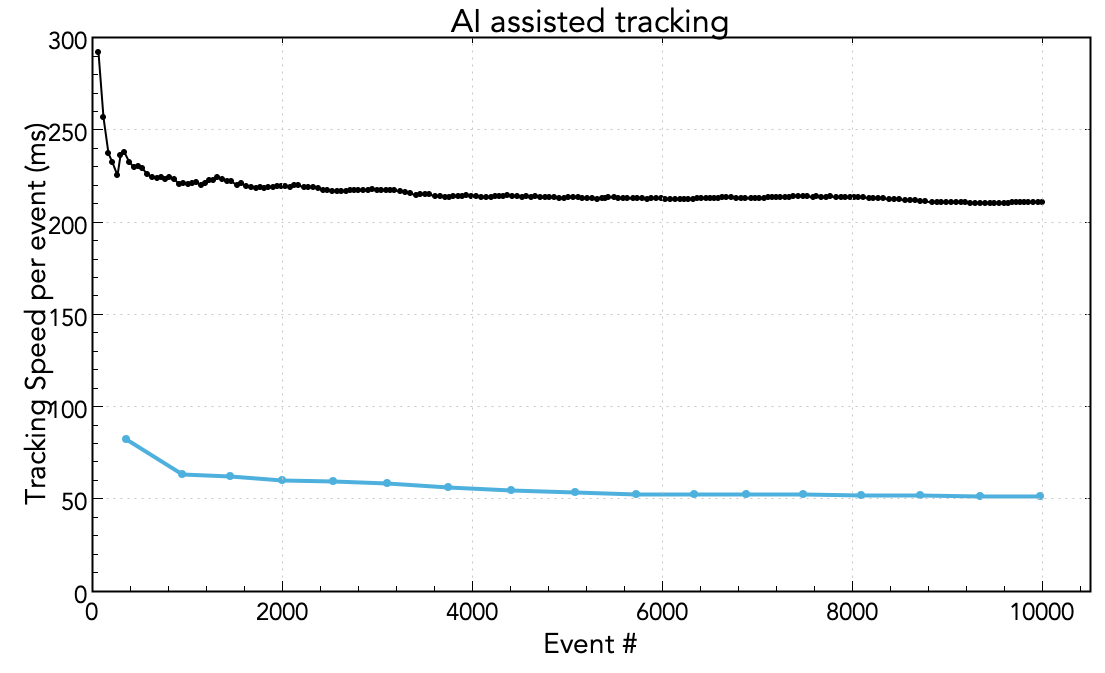
\includegraphics[width=0.45\textwidth]{pics/nn2.png}
\caption{Benchmark results of reconstruction speed for hit-based tracking. The (black) blue curve corresponds to
  the (non) artificial intelligence assisted reconstruction processing time as a function of event number.}
\label{fig:nn2}
\end{figure}

Implementing the neural network software into the CLAS12 reconstruction workflow is under development.
The second stage of the machine learning project will concentrate on efficiency improvements using artificial
intelligence assisted tracking.

\subsection{Improvement to Event Reconstruction}

The CLAS12 detector began beam operations for physics in early 2018 after a several month commissioning
phase. Since that time the event reconstruction code has continued to improve to meet issues as they have
arisen. However, the code and the framework are already performing well enough for advanced physics
analysis of the collected data to proceed. A broad survey of reconstruction results using the CLAS12
software framework and event reconstruction code are presented based on beam data in Ref.~\cite{clas12-nim}.
As might be expected, there are still areas where development, testing, and validations are in progress in
order to continue improvements. In this section, several areas of ongoing work are highlighted.

\subsubsection{Improvements to Central Tracking}

Improvements to tracking in the CVT are currently being studied. These include:

\begin{itemize}
\item improvements to the tracker geometry implementation and fitting algorithm - the combination of these
  code modifications is expected to improve the fit residuals, which are indicative of a bias in the current
  version of the code as seen through systematic shifts in their distributions;
\item implementation of geometrical distortions derived from detector alignment;
\item the use of the beam offset information (relative to the nominal beam $z$-axis) in the track fit initialization;
\item the use of SVT clusters instead of crosses in the seeding.
\end{itemize}

These updates aim at enhancing the robustness of the tracking algorithm and improving resolution and efficiency.

\subsubsection{Improvements to Time-of-Flight Reconstruction}

As discussed in Section~\ref{tof-sys}, the output of the time-of-flight reconstruction are hits that are used
as input to the Event Builder algorithms. The use of clusters for particles that go through two adjacent TOF
paddles (either in the FTOF or CTOF systems) is expected to yield improved timing resolution, as is combining
the hit times in FTOF for tracks that go through both forward counter hodoscopes as discussed in
Section~\ref{sec:tof-cluster}. A quantitative estimate of the timing resolution improvements and a validation of
the clustering algorithm are currently ongoing using on Monte Carlo simulations.

\subsection{Improvements to the Event Builder}

The matching of tracks to detector responses, either hits or clusters, is currently based on the distance of closest
approach between the tracks and the response coordinates. Improvements to this matching can be obtained using
track trajectories, i.e. intersections of the track with the relevant detector planes where the responses are reported.
The use of trajectories will reduce the uncertainty on the path length determination that relies on the response
coordinates. The use of timing information in the matching will reduce the effect of accidentals in high rates detectors
such as the HTCC.


